\documentclass{article}[12pt]
\usepackage[utf8]{inputenc}
\usepackage[T1]{fontenc}
\usepackage{array}
\usepackage{eqnarray}
\usepackage{caption}
\usepackage{amsmath}
\usepackage{amssymb}
\usepackage{comment}
\usepackage{hyperref}
\usepackage{fancybox}
\usepackage{gensymb}
\usepackage[english]{babel}
\usepackage{graphicx}
\usepackage{subcaption}
\usepackage{wrapfig}
\usepackage{xcolor}
\usepackage{mdframed}
\usepackage{titlepic}
\usepackage{titling}
\usepackage{listings}
\usepackage{placeins}
\usepackage{multicol}
\usepackage{authblk}
\usepackage{geometry}
\usepackage{float}
\geometry{hmargin=2.5cm,vmargin=2cm}
\usepackage{listings}
\usepackage{textcomp}
\usepackage{gensymb}
\usepackage{natbib}
\definecolor{codegreen}{rgb}{0,0.6,0}
\definecolor{codegray}{rgb}{0.5,0.5,0.5}
\definecolor{codepurple}{rgb}{0.58,0,0.82}
\definecolor{backcolour}{rgb}{0.95,0.95,0.92}
\hypersetup{
    colorlinks,
    linkcolor={blue!10!black},
    citecolor={blue!50!black},
    urlcolor={blue!50!black}
}
\usepackage{array,multirow,makecell}
\setcellgapes{1pt}
\makegapedcells
\newcolumntype{R}[1]{>{\raggedleft\arraybackslash }b{#1}}
\newcolumntype{L}[1]{>{\raggedright\arraybackslash }b{#1}}
\newcolumntype{C}[1]{>{\centering\arraybackslash }b{#1}}

\title{Electronic for measurement systems - Weighing scale}
\author{Pierre-Louis GIL and Youwan MAHÉ}
\date{Nov-Dec 2022, Grenoble-INP PHELMA}

\begin{document}

\maketitle
\tableofcontents
\newpage

\section{Sensor}
\paragraph{}
The main component behind weighing scales is the \emph{Straining Gauge}. Straining gauges are resistive sensors that are used to measure strain on an object. The resistive part is usually made of metal and glued to an insulating adhesive surface such as cyanoacrylate. Since the variation of resistance is  small, it is very common to use a Wheatstone bridge configuration to transform the variation of resistance in a differential voltage.
\subsection{Gauge factor and measurand}
\paragraph{}
The Gauge Factor $GF$ is a quantity used to describe the sensitivity of a strain gauge.
\begin{equation}
GF=\dfrac{\Delta R/R}{\epsilon}
\end{equation}
\begin{itemize}
\item $\epsilon$ is the strain (ration between length under stress and length at rest)
\item $\Delta R$ The variation of resistance
\item $R$ Resistance at rest
\end{itemize}
Using the Wheatstone bridge, we convert the $\Delta R$ in a differential voltage $V_{sensor}$.
\begin{figure}[H]
\centering
\begin{subfigure}{.5\textwidth}
  \centering
  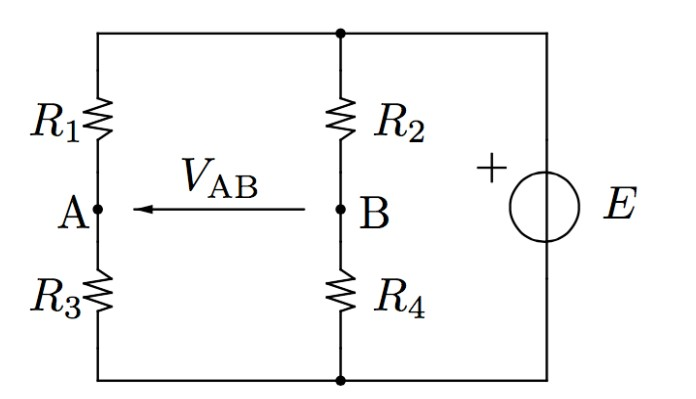
\includegraphics[width=.8\linewidth]{figures/wheatstone.jpg}
  \caption{Wheatstone's bridge schematic}
  \label{fig:Wheatstone}
\end{subfigure}%
\begin{subfigure}{.5\textwidth}
  \centering
  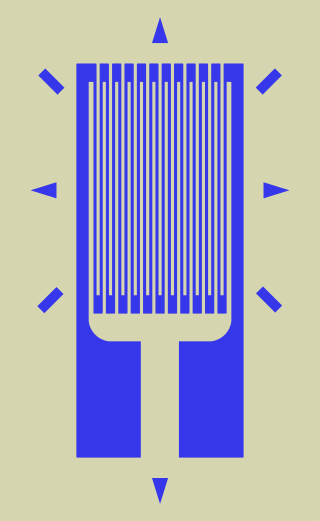
\includegraphics[width=.4\linewidth]{figures/Strain_gauge.png}
  \caption{Staining gauge}
  \label{fig:sub2}
\end{subfigure}
\caption{}
\label{fig:test}
\end{figure}
\begin{equation}
V_{sensor}=\dfrac{GF \epsilon}{4}E
\end{equation}
\begin{itemize}
\item $E$ is the bridge voltage at rest
\item $GF$ the gauge factor
\item $\epsilon$ The strain
\item $V_{sensor}$ the differential voltage
\end{itemize}
\paragraph{}
Our strain gauge is the model DF2S made by HBM (Hottinger Baldwin Messtechnik GmbH). It comes directly with an inbuilt Wheatstone bridge made with 1000$\Omega$ strain gauges. The maximum load we will use for this project is 1kg. We measured the characteristic of our sensor with the help of known masses and a high sensitivity digital multimeter from fluke. The result is shown in \ref{fig:beforeamp}.
\begin{figure}[H]
	\centering
	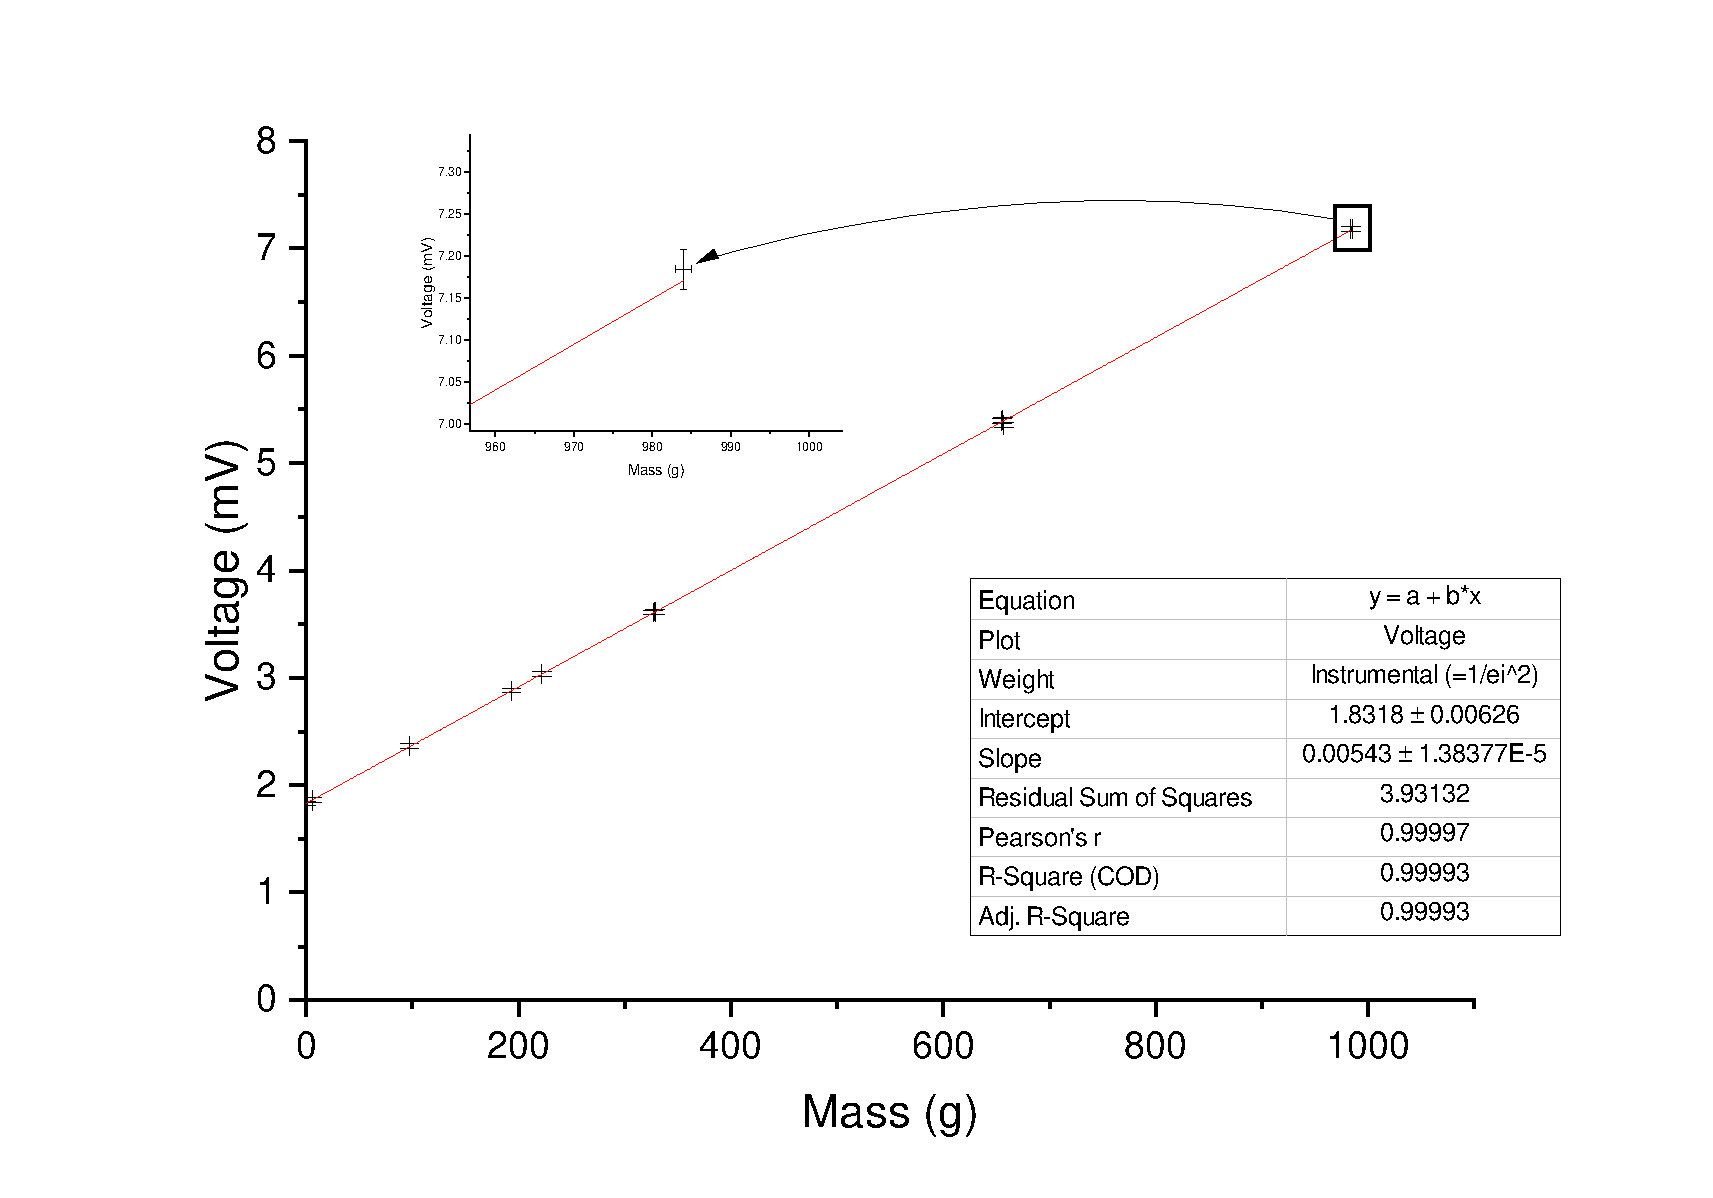
\includegraphics[width=\textwidth]{figures/beforeamp.pdf}
	\caption{Characteristic of our sensor before any amplification with the Wheatstone bridge exited at $E=3.33V$}
	\label{fig:beforeamp}
\end{figure}

%----------------------------------------------------------------%
\section{Amplifier}
\subsection{Theory of operation}
\paragraph{}
As seen in figure \ref{fig:beforeamp} he signal that outputs the Wheatstone bridge is a weak differential signal (~mV).
\paragraph{}
We need to amplify it in order to get an acceptable signal for the Analog to Digital Converter.
The amplification is done by using a 3 AOP differential amplifier.
\begin{figure}[H]
    \centering
    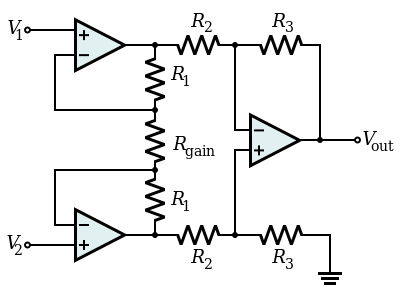
\includegraphics[width = .4\textwidth]{figures/3AOP_differential_amplifier.png}
    \caption{3 Amp op differential amplifier}
    \label{fig:3OpAmp}
\end{figure}
The difference of potential between the two branches is amplified according to this formula.
\begin{equation}
    \dfrac{V_{out}}{V_1-V_2}=(1+\dfrac{2R_1}{R_{gain}})\dfrac{R_3}{R_2}
\end{equation}
\subsection{Gain of the amplifier according to documentation}
In our case, we could only change the value of Rg as the differential amplifier is a component and not a circuit we had to make. The gain of this amplifier is calculated as follow:
\begin{equation}
    G=5+\dfrac{80000}{R_g}
\end{equation}
Knowing the maximum value that this amplifier can output as well as the maximum differential voltage of the Wheatsone bridge, it is possible to calculate the maximum gain authorised for our scale.
\begin{equation}
    Rg= \dfrac{80000}{G-5}
    \label{equ:rg}
\end{equation}
\begin{itemize}
    \item $R_g$ is the value of the gain resistance in $k\Omega$
    \item $G$ is the gain of the amplifier
    \item $80000$ is a value in $k\Omega$
\end{itemize}
The maximum mass we want to be able to measure is 1kg.
Using the linear regression extrapolated from the Wheatstone bridge (figure \ref{fig:Wheatstone}) we obtain that the differential voltage for 1kg is 7.26 mV.
As 3.33 V is the maximum output value of our differential we obtain a maximum gain of 459.
Using (\ref{equ:rg}) we obtain a resistor of 176 $\Omega$. We do not posses such resistor so we chose the closest higher resistor value we have at our disposal to not saturate.
The value of Rg is 220 $\Omega$ which correspond to a gain of 369.
%insert figure differential amplifier output before correction
We can see that the signal is being correctly amplified, there is no saturation. However, we can observe an offset that can be caused by the strain of the platform on the strain gauge.
In order to correct this offset, we added a resistor in the Wheatstone bridge.
%insert figure of modified Wheatstone bridge
This new resistor forms an equivalent resistor with R4 which helps us to readjust the potential in the node B to match the potential in node A so that the offset is negated.
We want to adjust around 0.002 mV so our resistor should be around 1M$\Omega$.
The value 470k$\Omega$ was empirically chosen.
We obtain the following results
%insert figure differential amplifier output after correction
%ajouter les limites

%----------------------------------------------------------------%
\section{Analog to Digital Converter}
\subsection{Theory of operation}
\paragraph{}
Now that the signal is amplified, we can convert it into a digital signal via an Analog to Digital Converter (ADC).
The ADC is a $\Delta$$\Sigma$-ADC which means that the voltage value is converted into a linear amount of pulses during a period P. 
The higher the voltage the more pulses it outputs.
\paragraph{}
As seen in the schematic below, if we consider the signal to be constant, the integrator transforms it into a linear function.
Once that function reaches a threshold, a pulse is emitted, then each pulse is added on the output signal and by counting the amount of pulse (one pulse is equivalent to one quantum of voltage) it is possible to find the voltage.\\
\begin{figure}[H]
    \centering
    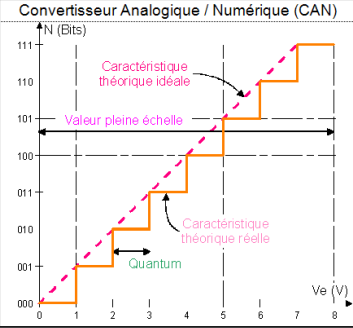
\includegraphics[width=.4\textwidth]{figures/CAN.png}
    \caption{Analogue to digital conversion modelized by a step function}
    \label{fig:CAN_step}
\end{figure}
We can have $2^{16}$ values from 0 to 2.048 V so our quantum is 31.2 $\mu$V.
\begin{figure}[H]
    \centering
    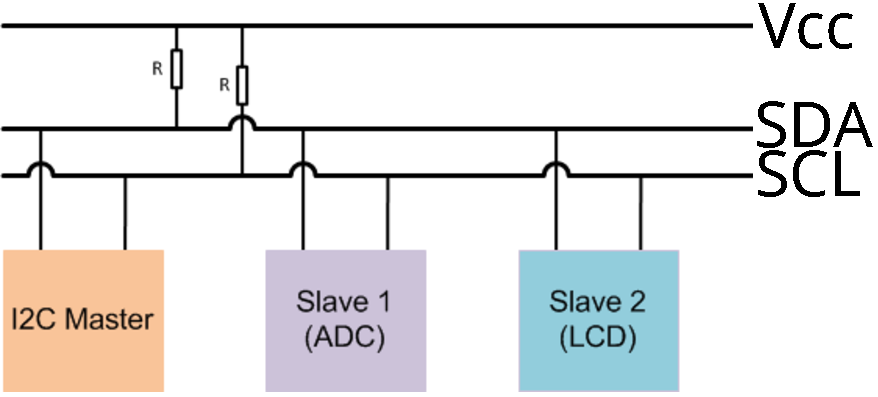
\includegraphics[width=\textwidth]{figures/i2c_diagram.pdf}
    \caption{$I^2C$ schematic}
    \label{fig:i2c_diagram}
\end{figure}
The ADC uses the $I^2C$ protocol to convey information to the mother board. 
The $I^2C$ protocol revolves around two wires that connects one master (the mother board here) and slaves (the ADC). 
One transfer data while the clock signal is in the other.
Each slave has an address that the master uses to call it whenever it needs it.
Each bit of data bus is given by a voltage, if there is 0V it is considered to be 0 and if there is a voltage it is a 1,
The signal created is now a logical signal that can be translated by the master.
%insert bus data schematic
The signal is composed of a start bit then the address of the slave in binary then the slave respond via a bit called ACK.
The clock signal is used to read the data sent.
It is thus possible to have more than one slave with only two wires (We wont use this feature here).
In order to have these two different voltages, we use two resistor connected to Vcc and the wires.
Each wire can be connected to the ground so that the voltage can be 0V (bit 0) or not 0V (bit 1), the pull up resistor prevent short-circuiting and fix the bit to 1 when no one send data through the wires.
%limits here
%----------------------------------------------------------------%
\section{Noise reduction}
\paragraph{}
A lab is isolated from a lot of external noise. In order to reinforce the noise reduction capability of our weighting scale, we must add some noise sources to see and reduce the effects. We will be focusing on two noise sources : a vibration generator and an electromagnetic noise generator.
\subsection{Mechanical vibrations}
\paragraph{}
A small electric motor with a mass is added near the sensor. A non-symmetrical mass is placed on the rotor in order to create a distance between the centre of rotation and the gravity centre of the mass. When rotating, this device produces vibrations. Using the stroboscopic effect of our smartphone camera (at 60 frames per second) we set the motor speed at 60Hz.
\paragraph{}
The periodic nature of the synthetic noise is easily quantified using Fast Fourrier Transform algorithm on a long enough signal sample (1s in our case).
The results are the following :
\begin{figure}[H]
\centering
\begin{subfigure}{.5\textwidth}
  \centering
  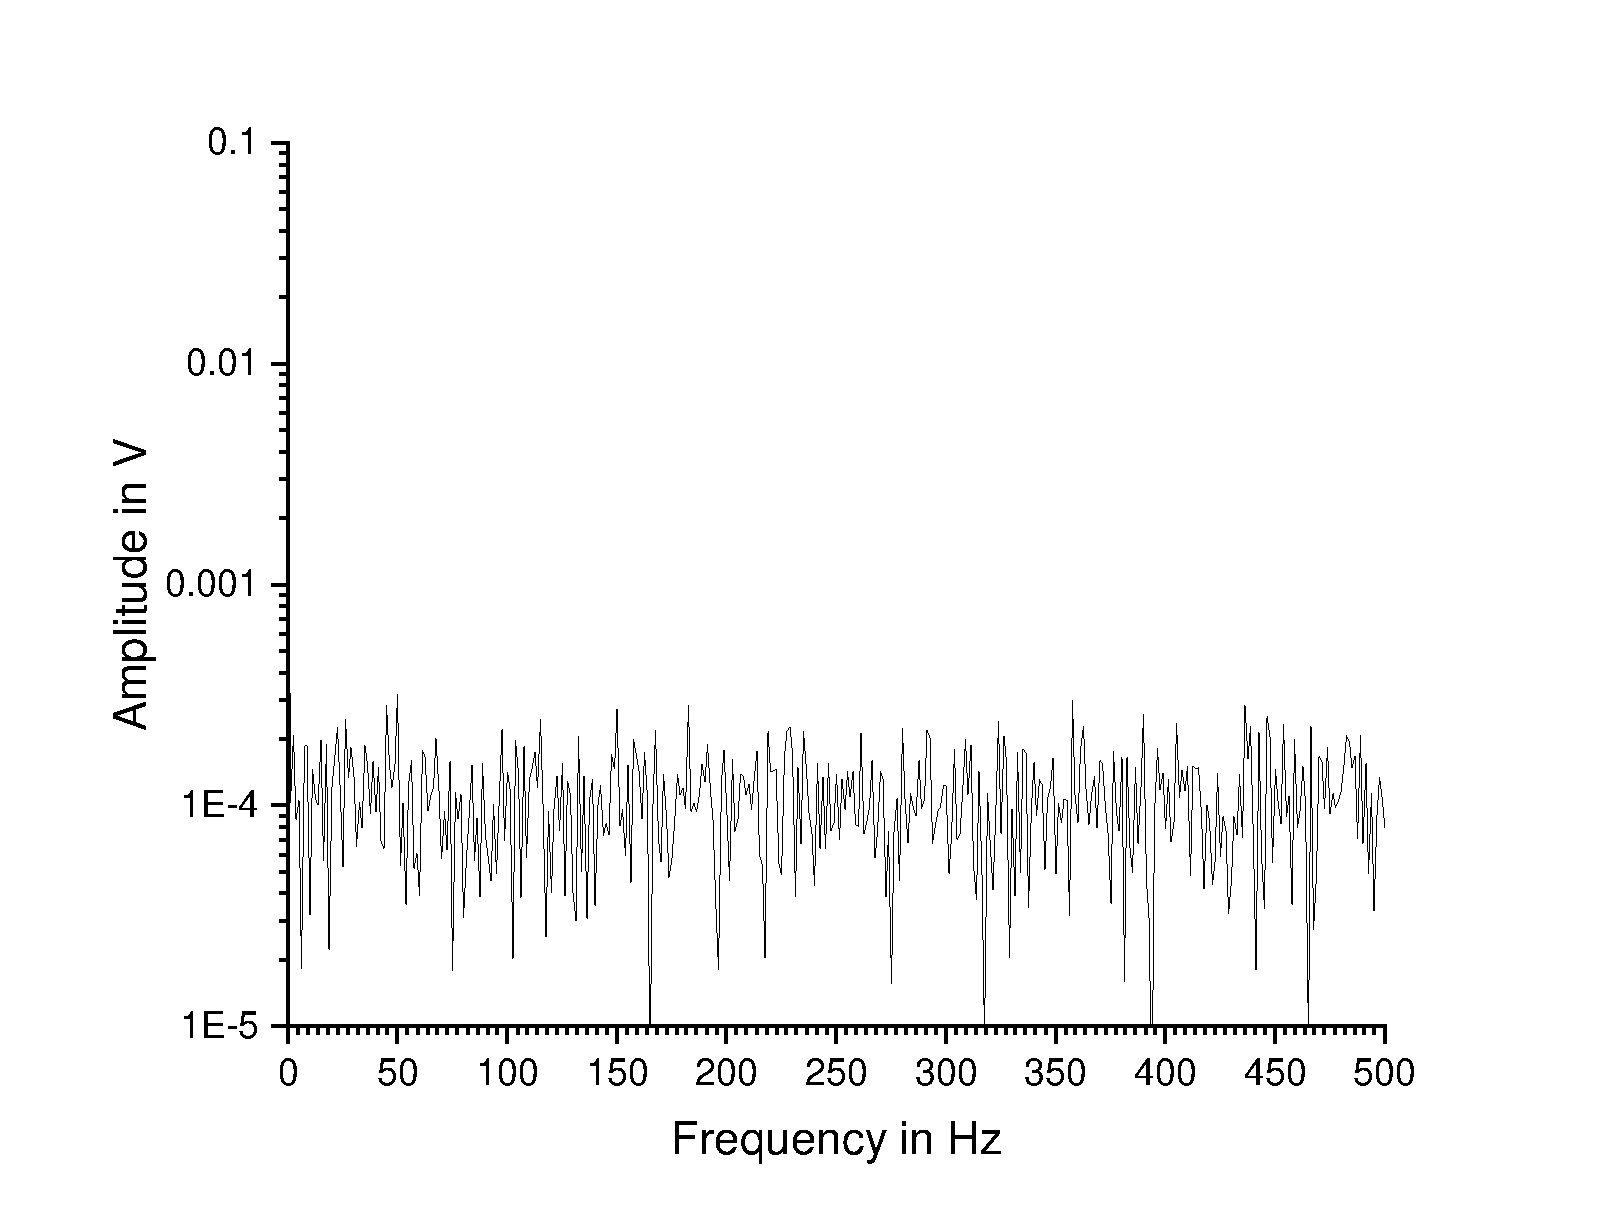
\includegraphics[width=\linewidth]{figures/nomotornofilter.pdf}
  \caption{FFT of the recovered signal before digitalization\\ without the motor}
  \label{fig:nomotornofilter}
\end{subfigure}%
\begin{subfigure}{.5\textwidth}
  \centering
  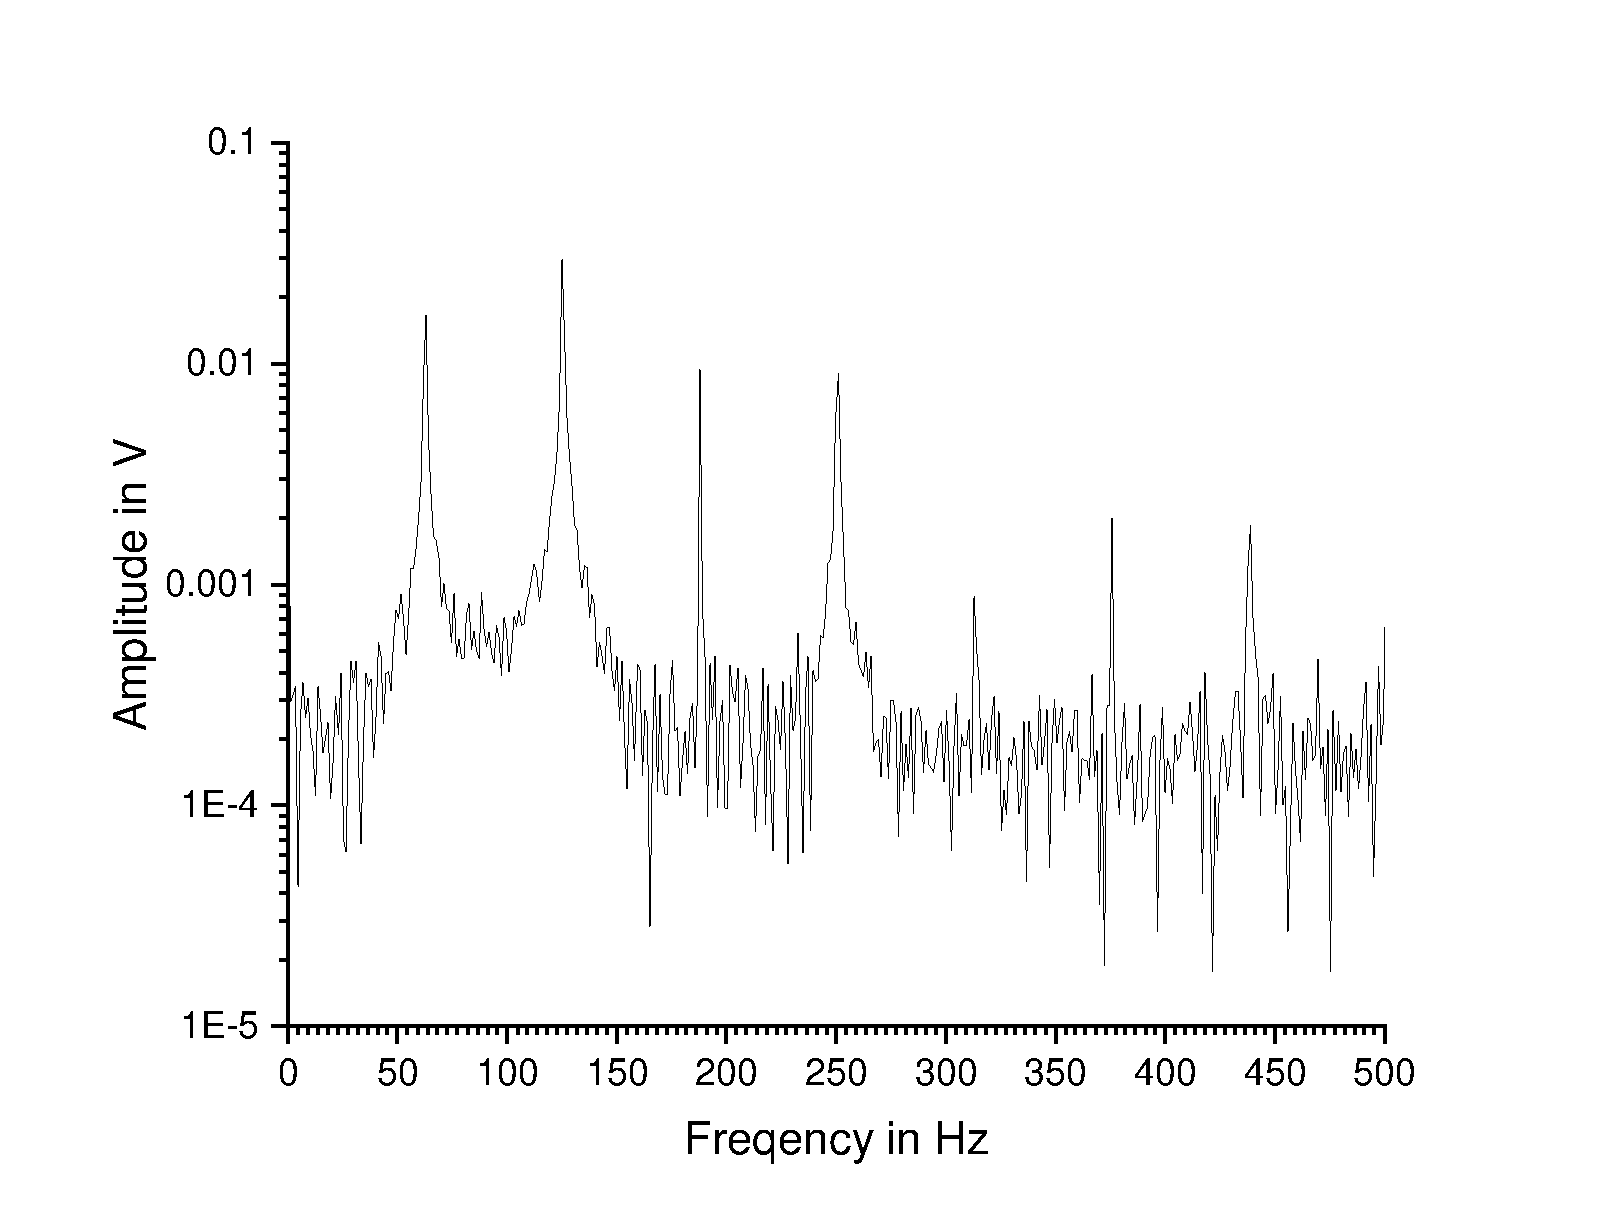
\includegraphics[width=\linewidth]{figures/motornofilter.pdf}
  \caption{FFT of the recovered signal before digitalisation\\ with the motor at 60 rounds per second}
  \label{fig:motornofilter}
\end{subfigure}
\caption{}
\label{fig:nofilterFFT}
\end{figure}
Figure \ref{fig:nofilterFFT} shows an evident spectral contribution of the vibration device we added. In addition, we observed the standard deviation of a weigh measurement. We acquired more than 30 values in each cases for determination of an experimental standard variation using the SD formula of our data processing software : $s = \sqrt{\frac{1}{n-1} \sum_{i=1}^n (x_i - \overline{x})^2}$. \\
\begin{center}
\begin{tabular}{|c|c|}
    \hline
    Without motor & With Motor \\
    \hline
     $1.20$mV & $3.39$mV \\
    \hline
\end{tabular}
\end{center}
\paragraph{}
Since the usefull part of the signal is only in the DC componenent. A Low-Pass filter should eliminate the disturbance while keeping the information in the signal.
\paragraph{}
In accordance with the available components, an RC filter ($1^{st}$ order) with a cuttof frequency of $0.8Hz$ is added to the circuit. Same measurements are made with after the filter is soldered on the board. Results are the following : 
\begin{figure}[H]
\centering
\begin{subfigure}{.5\textwidth}
  \centering
  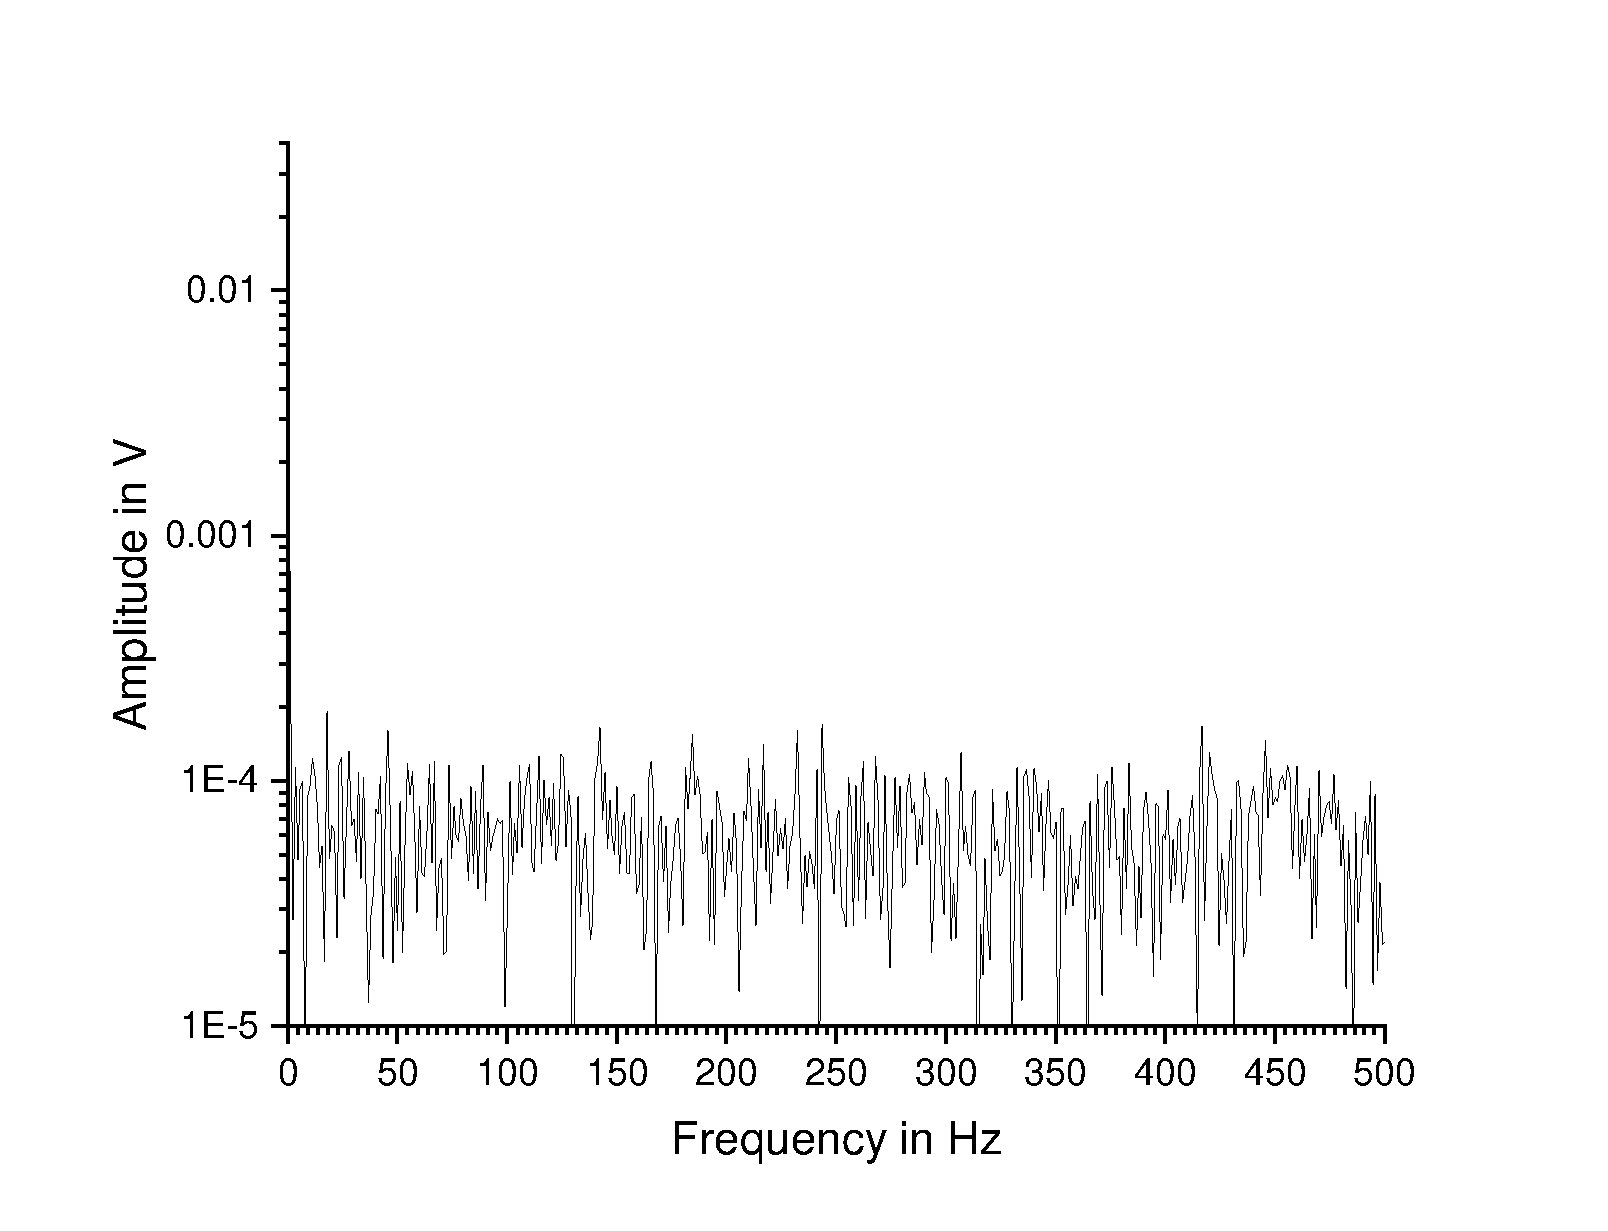
\includegraphics[width=\linewidth]{figures/nomotorfilter.pdf}
  \caption{FFT of the recovered signal before digitalization\\ without the motor}
  \label{fig:nomotornofilter2}
\end{subfigure}%
\begin{subfigure}{.5\textwidth}
  \centering
  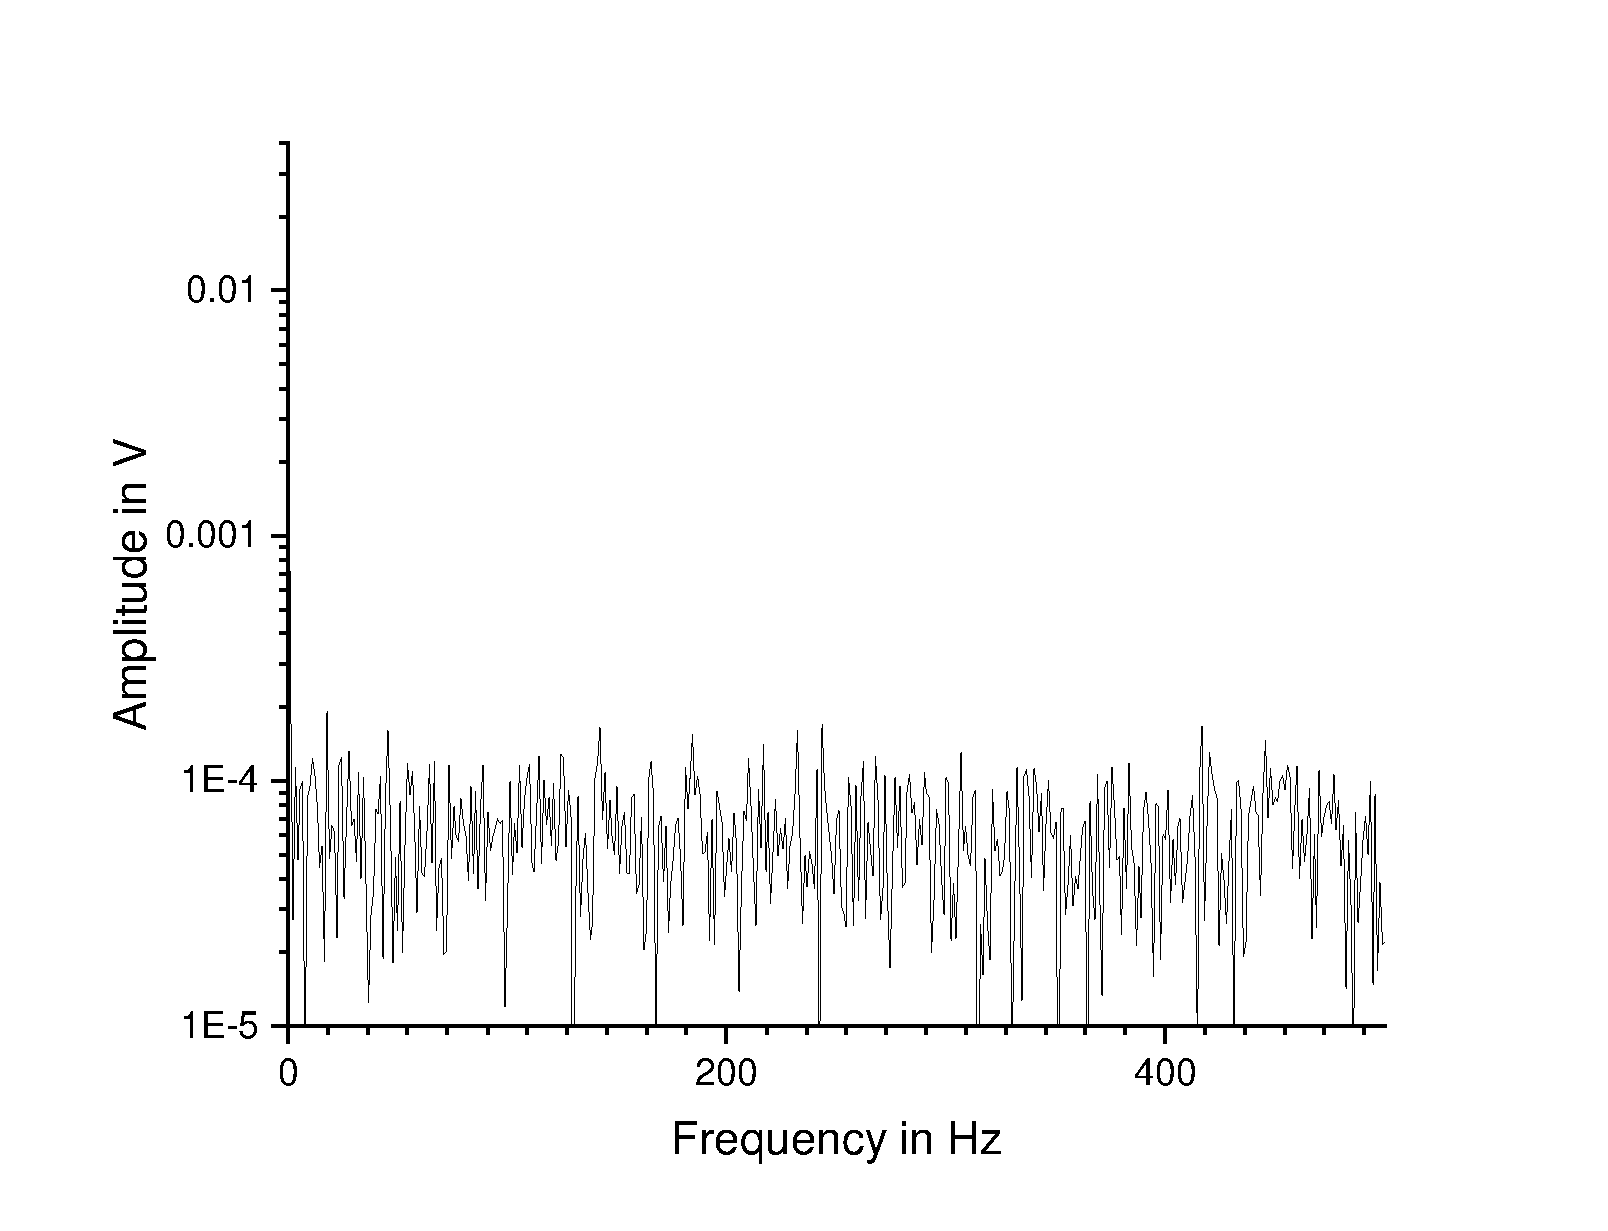
\includegraphics[width=\linewidth]{figures/motorfilter.pdf}
  \caption{FFT of the recovered signal before digitalisation\\ with the motor at 60 rounds per second}
  \label{fig:motornofilter2}
\end{subfigure}
\caption{With the RC Low-Pass filter}
\label{fig:filterFFT}
\end{figure}
Figure \ref{fig:filterFFT} shows the absence of AC component noise in our signal. Howerver, with the filter the stabilisation of the value takes more time. We must wait $3\tau$ to get a stable value. On the other hand, the displayed value seemed more stable. The same standard deviation measurement was made and the results showed a reduced variance of both values.
\begin{center}
\begin{tabular}{|c|c|}
    \hline
    Without motor & With Motor \\
    \hline
     $0.095$mV & $0.109$mV \\
    \hline
\end{tabular}
\end{center}
The Motor contribution to the variance of the measurement system is completely wiped thanks to the low pass filter.
\subsection{Electromagnetic noise}
Electric motors are made with carbon brushes to make an electrical contact between the static wires and the moving parts. Because the contact is not always perfect, some sparks may occur randomly in the enclosure of the motor. Sparks can be assimilated as electromagnetic Diracs of high intensity. Using a large enough time-span, we can observe the sparks being transmitted by electromagnetic waves to the copper of the printed circuit board. The time span must not be too wide because the probability of the oscilloscope skipping a spark between two points increases with the sampling frequency. Figure \ref{fig:sparks} show some sparks acquired on the oscilloscope.
\begin{figure}[H]
    \centering
    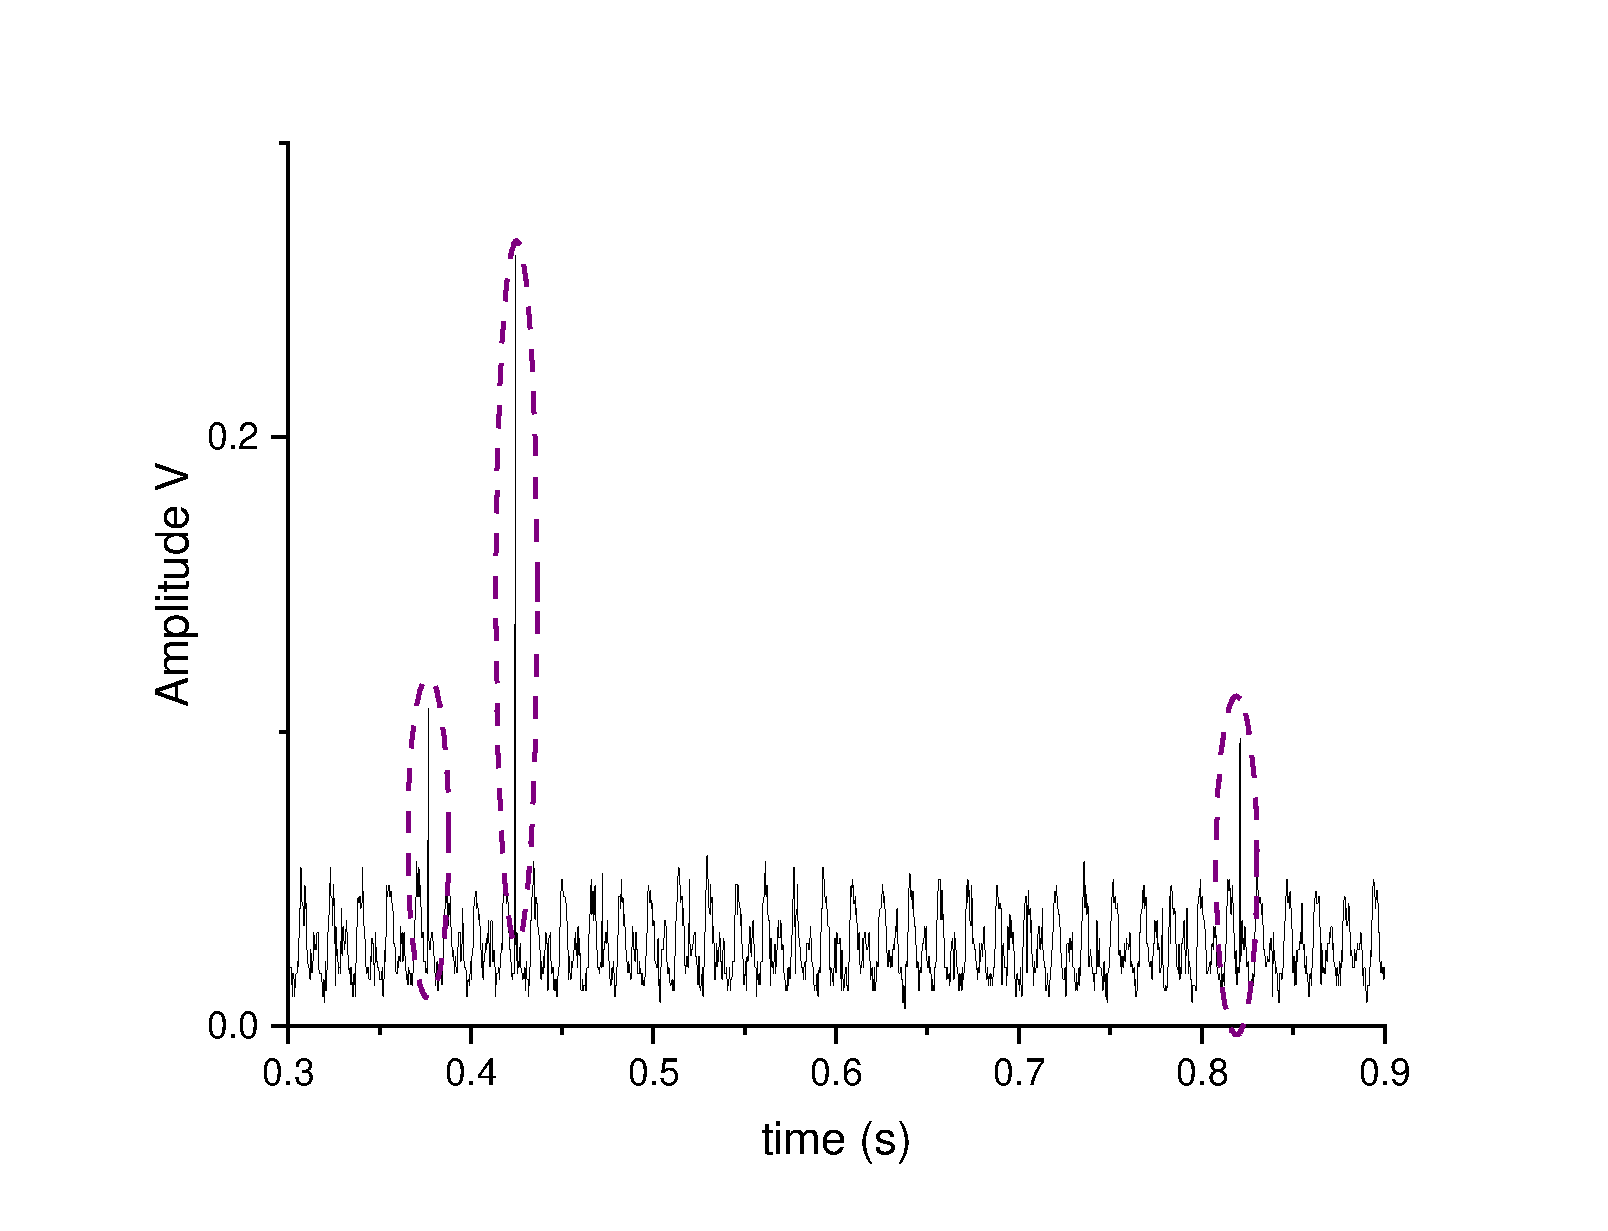
\includegraphics[width=0.6\textwidth]{figures/sparks.pdf}
    \caption{in Violet dashes : EM Sparks triggered by the brushes of the electric motor}
    \label{fig:sparks}
\end{figure}
\paragraph{}
To reduce the sparks effect, a proof-of-concept faraday cage was made using steel plates. 
\begin{figure}[H]
\centering
\begin{subfigure}{.5\textwidth}
  \centering
  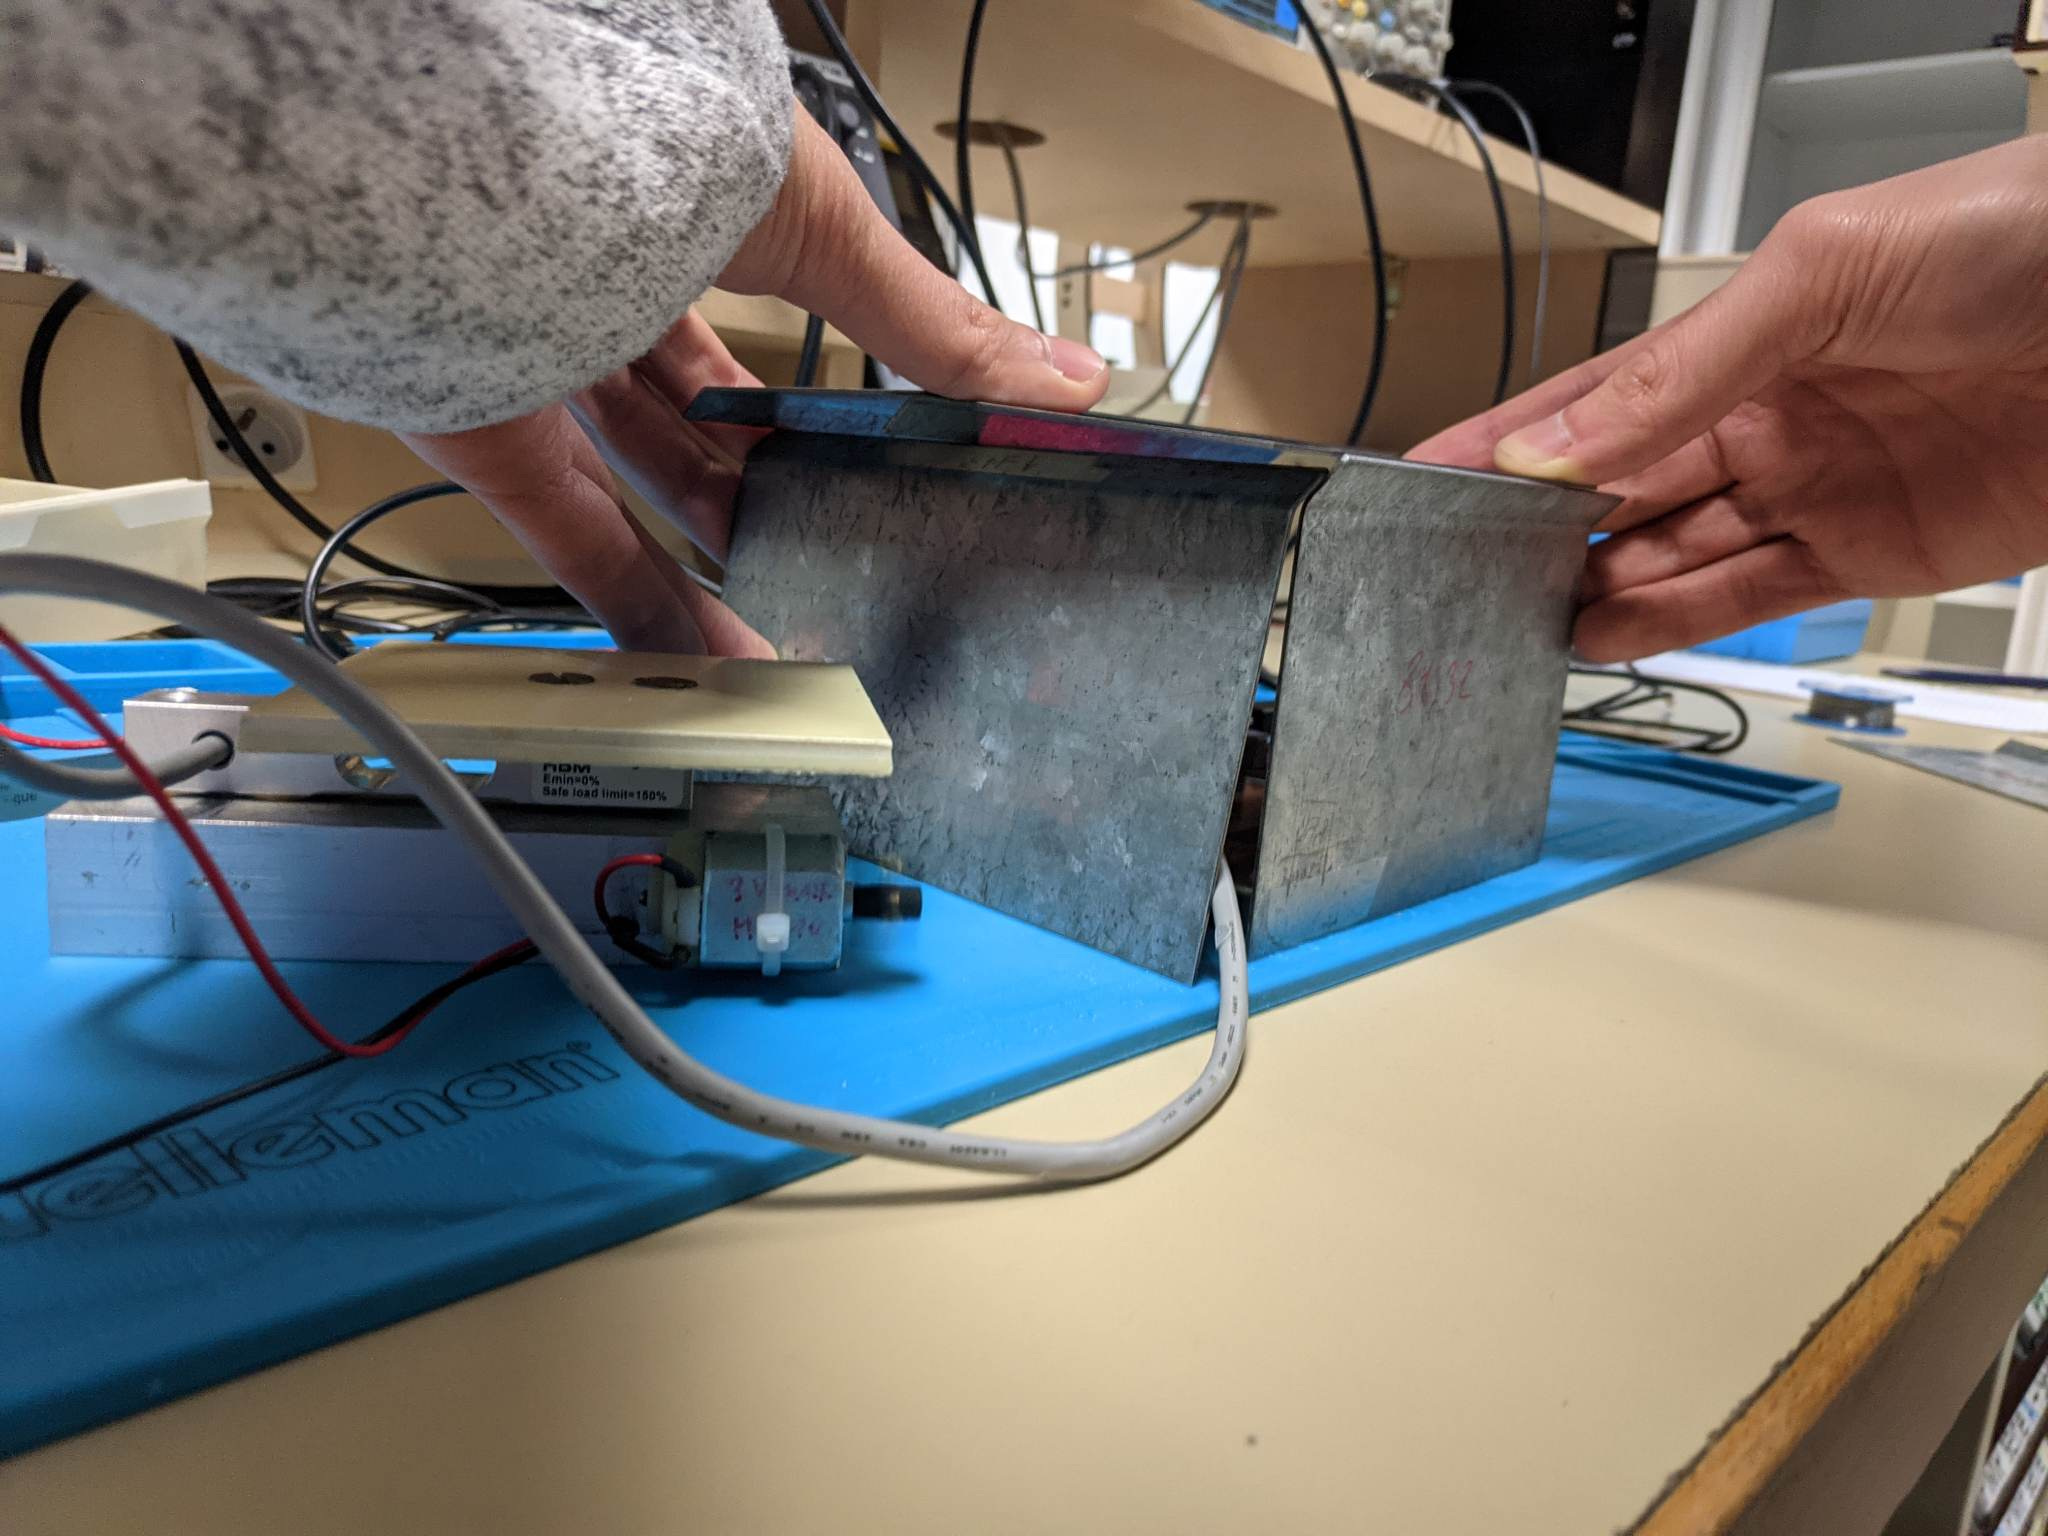
\includegraphics[width=\linewidth]{figures/faraday.jpg}
  \caption{Picture of the faraday cage setup arround the printed circuit board}
  \label{fig:faradaypic}
\end{subfigure}%
\begin{subfigure}{.5\textwidth}
  \centering
  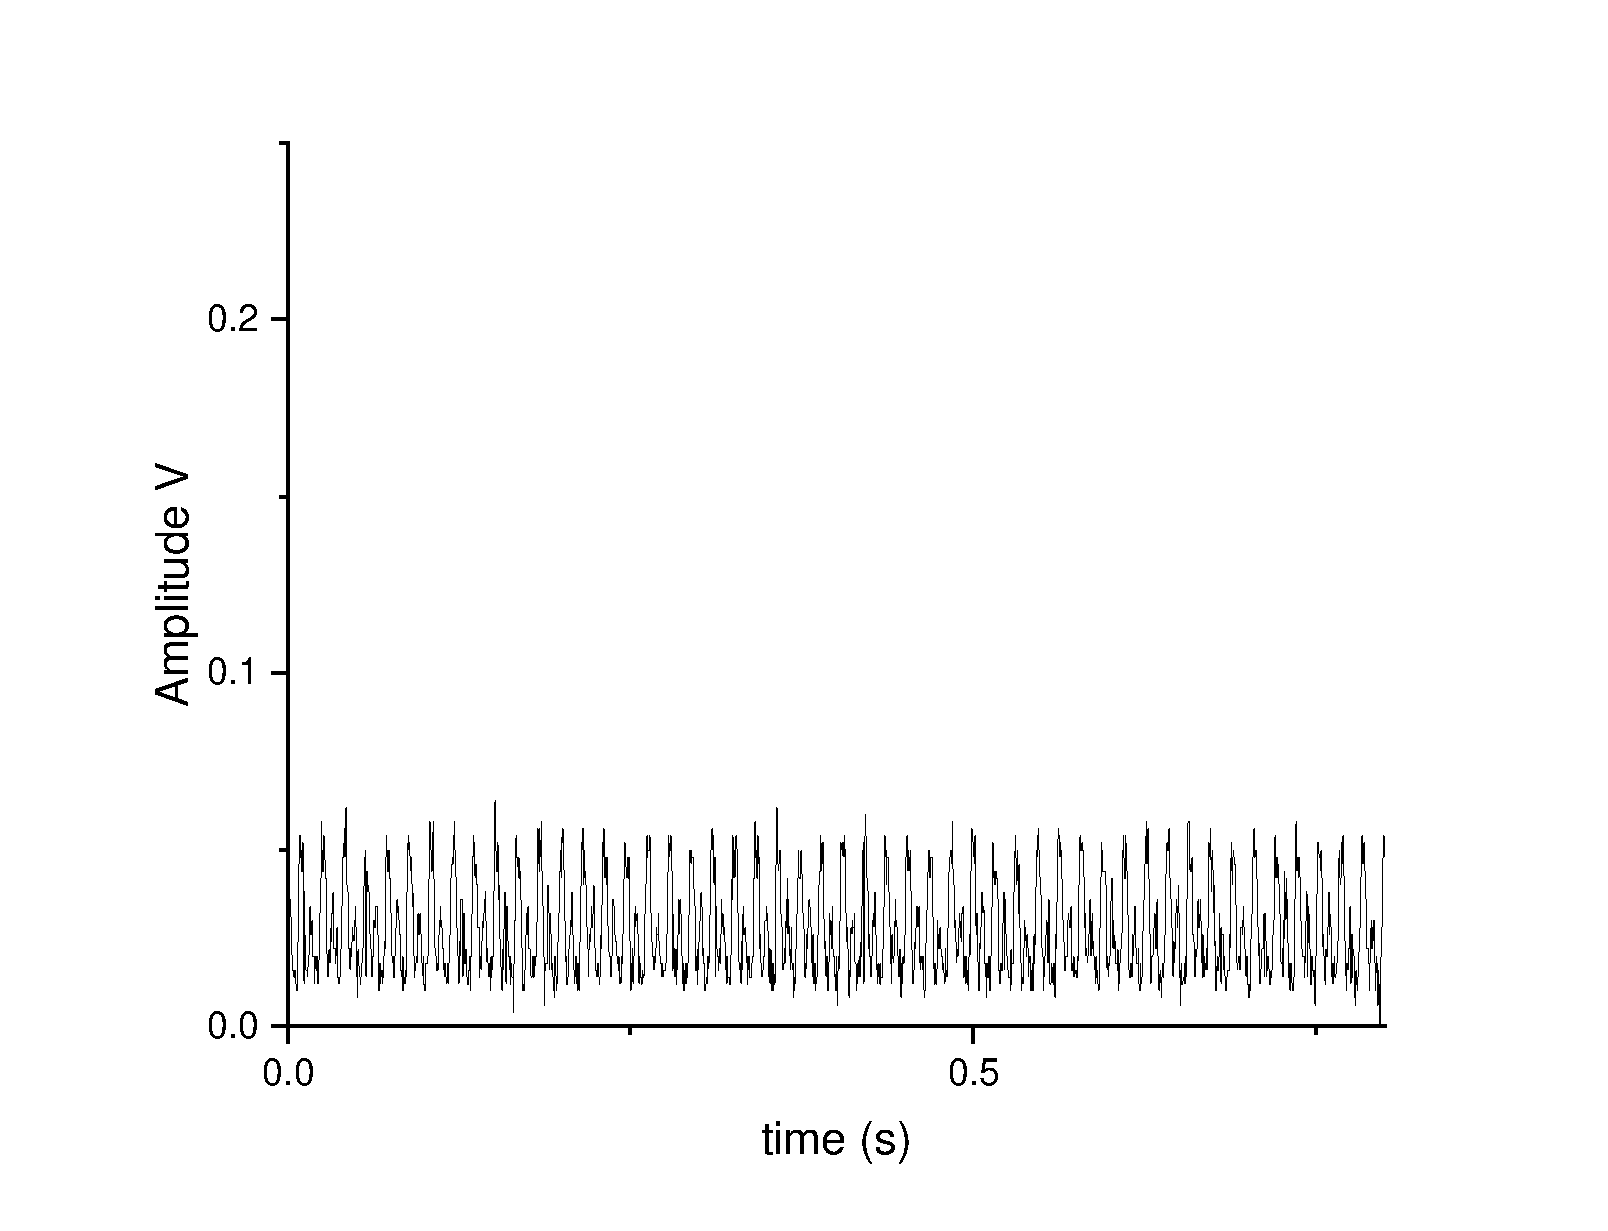
\includegraphics[width=\linewidth]{figures/faraday.pdf}
  \caption{Signal with absence of sparks}
  \label{fig:faradaysig}
\end{subfigure}
\caption{}
\label{fig:faraday}
\end{figure}
\paragraph{}
The data proves that a metallic shield provide good insulation against such EM disturbances. We could consider integrating it in the final product.
%----------------------------------------------------------------%
\section{Error Budget}
\paragraph{}
The prototype is now fully completed. The layout of the PCB is drawn on figure \ref{fig:layout}
\begin{figure}[H]
    \centering
    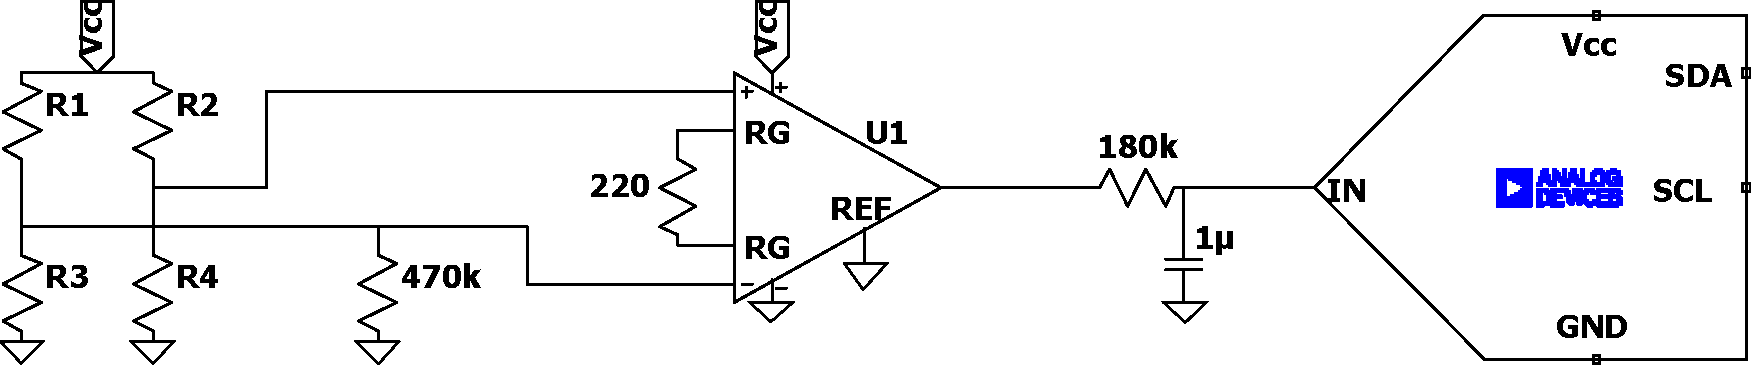
\includegraphics[width=\textwidth]{figures/layout.pdf}
    \caption{Layout of our printed circuit board}
    \label{fig:layout}
\end{figure}
The thermal noise or Johnson–Nyquist noise affects only resistive components. The RMS Voltage resulting of the noise is given by :
\begin{equation}
    V_{noise}=\sqrt{4Rk_bT\Delta f}
\end{equation}
\begin{itemize}
    \item $\Delta f$ Bandwidth in Hertz
    \item $R$ Resistance in Ohm
    \item $k_b$ Boltzman's Constant : $1.380649.10^{-23} J.K^{-1}$ 
    \item $T$ Temperature in Kelvin
\end{itemize}

%INSERT BuDGET ERROR HERE
The differential amplifier can be modelled this way to take into account the different imperfections of the amplifier.
The values can be found in the amplifier's datasheet.
Each component of the error can be calculated separately then the squared values can be summed up to obtain the total error budget of the system.
%insert schematic
\begin{itemize}
    \item $V_{INoise+}$ = 0.21 nV
    \item $V_{INoise-}$ = 0.21 nV
    \item $V_{Bias+}$ = 14 $\mu$V
    \item $V_{Bias-}$ = 14 $\mu$V
    \item $V_{Noise}$ = 0.35 $\mu$V
    \item $V_{OFS}$ = 164 $\mu$V
    \item $V_{IOFS}$ = 1.25 $\mu$V
\end{itemize}
The total error budget
We can also describe the error in terms of affected quantum. In our case, the 16 bit resolution of the conversion devices allows us to neglect the quantification error with respect to the electrical noise. We can therefore calculate the amount of noise in quantum units, and we will determine the Signal to noise ratio between number of affected quantum and $2^{16}$ bits.
%----------------------------------------------------------------%
\section{Conclusion}
\subsection{Final calibration of the weighting scale}
\paragraph{}
\begin{figure}[H]
    \centering
    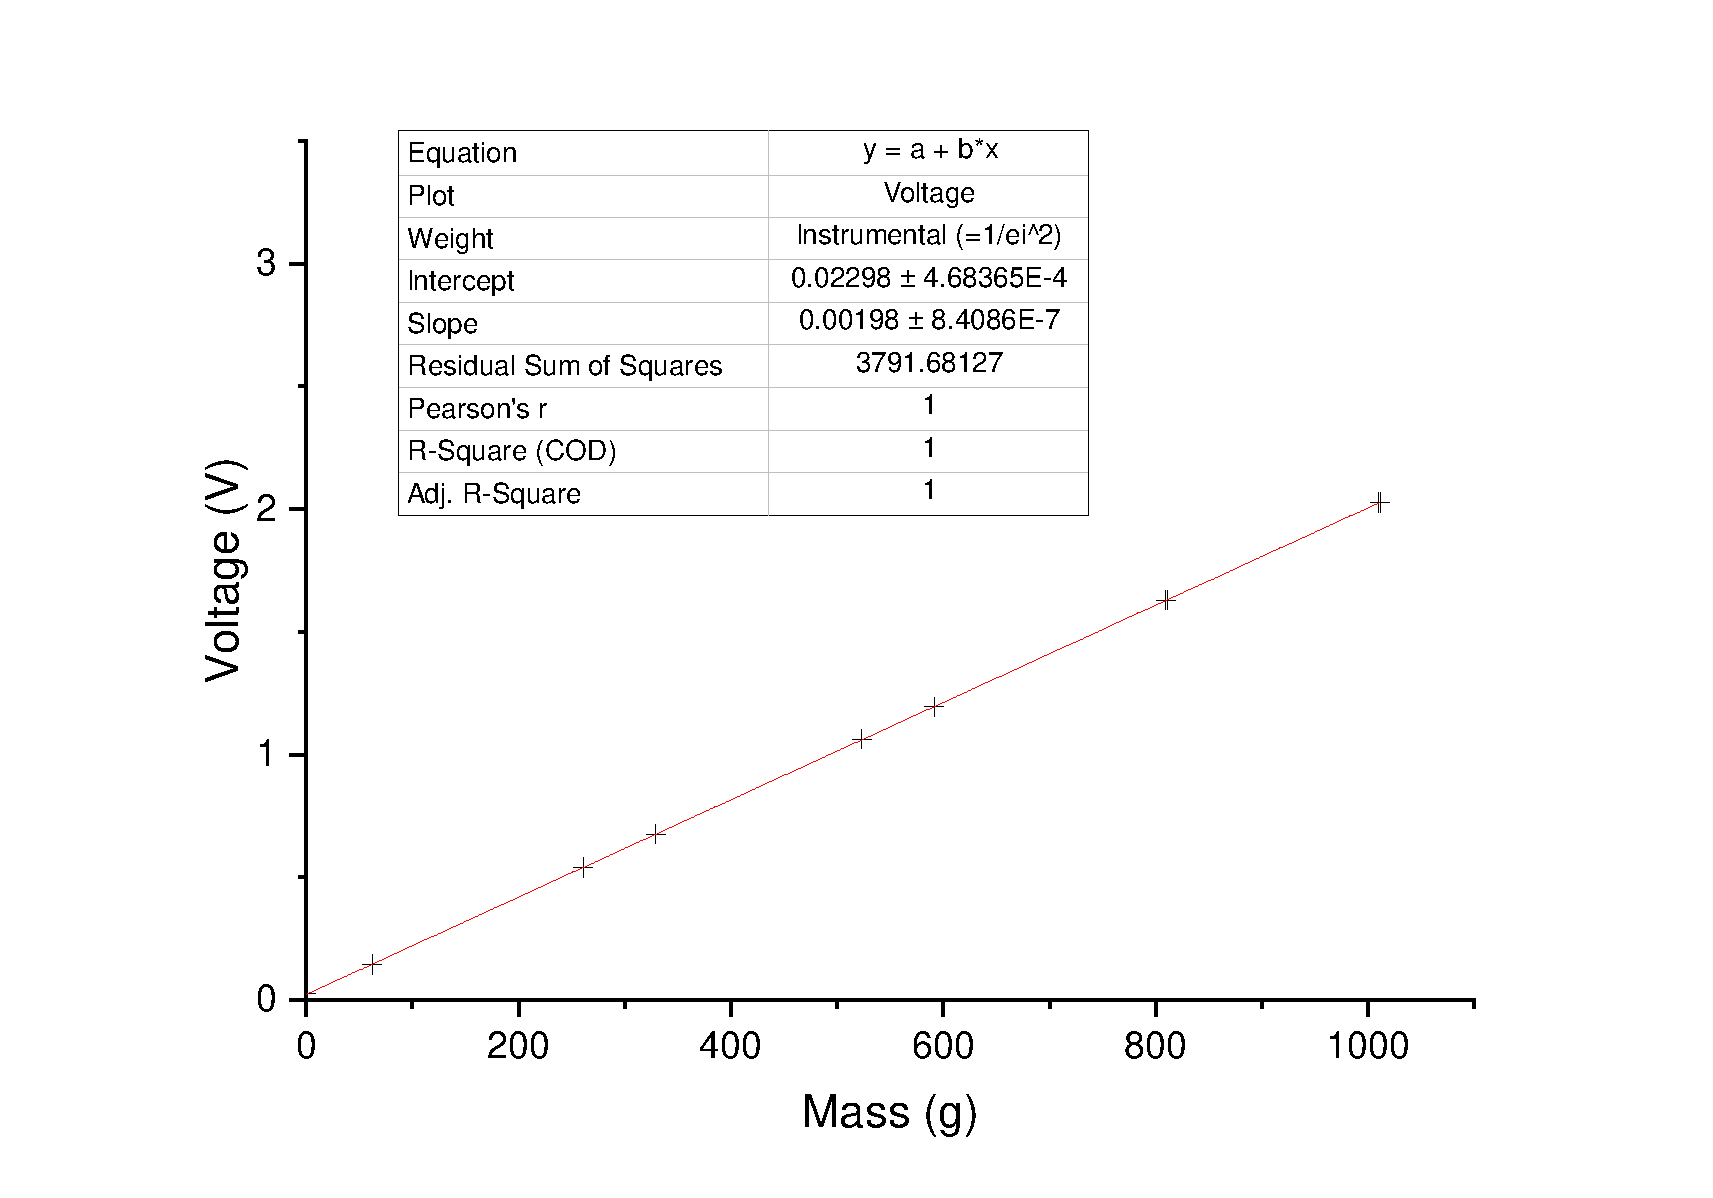
\includegraphics[width=.8\textwidth]{figures/calibr.pdf}
    \caption{Final calibration of or measurement system}
    \label{fig:final_calibration}
\end{figure}

\newpage
%----------------------------------------------------------------%
\section{Bibliography}
\bibliography{biblio}
\bibliographystyle{alpha}
\end{document}
